\chapter{The Standard Model of Particle Physics}

%\epigraph{\textit{So it goes...}}{---Kurt Vonnegut, \textit{Slaughterhouse
%		Five}}
	
%\epigraph{\textit{Science is a miracle.}}{--Ron Swanson}

\epigraph{\textit{If you wish to make an apple pie from scratch, you must first invent the universe.}}{--Carl Sagan, \textit{Cosmos: A Personal Voyage}}


As it stands, what has become known as the `Standard Model (SM) of Particle Physics'
is nothing less than one of the greatest achievments of mankind, due to both
the magnitude by which it has changed our perception of the underlying
nature of the universe and to the clever methods and tinkerings by which this
nature was unveiled by many clever physicists whose history has become veritable lore.
In terms of imagination and insight, it is second only to the special and general theories of relativity --
though the fields are nevertheless intricately intertwined.
%{\color{red}{The latter, though, being put forth by essentially a single person and the latter by a great many...}}.

Not considering the scientific progress made in the $18^{th}$ and $19^{th}$ centuries, and
ignoring the ancient Greeks despite their fabled invention of atomic theory,
the physical insights and major work that led to the current picture of elementary particle
physics described by the SM began with the \textit{annus mirabilis} papers of Albert
Einstein in the year 1905~\cite{einsteinPEE,einsteinSpecial,einsteinEnergyMass}.
In these papers, Einstein was able to shed light on the quantization of electromagnetic
radiation (building off of the seminal work of Max Planck~\cite{planckBlackBody})
and introduce the special theory of relativity.
These works laid the conceptual
and philosophical groundwork for the major breakthroughs in fundamental physics
of $20^{th}$ century physics: from the `old quantum theory' of Bohr and Sommerfeld
in the early 1900's to the equivalent wavefunction and matrix-mechanics formulations
of Schr{\"o}dinger and Heisenberg that
coalesced into `modern' quantum mechanics in the mid-1920's.
The modern approach, non-relativistic at its heart, provided a sufficient mathematical
and interpretable framework in which to work and match predictions to observed phenomena, old
and new. It has for the most part remained unchanged and is the quantum mechanics that is taught to
students at both the undergraduate and graduate level to this very day.
It is the theory that has since revolutionised all aspects of the physical sciences and
technologies that dictate our everyday-lives.
In the mid-1920's, however, despite
large efforts put forth by the forbears of modern quantum mechanics, the quantum-mechanical
world had yet to be made consistent with Einstein's theory of relativity --- a requirement
that must be met for all consistent physical theories of nature.
It was the insight of Paul Dirac who was finally able to successfully
marry the theory of the quantum with that of relativity when he introduced
his relativistic quantum-mechanical treatment of the electron in 1927 and 1928~\cite{diracEquation,Dirac:1927dy}.\footnote{
A complete history of the people and ideas involved in the development of the modern
theory of Quantum Mechanics can be found in references ~\cite{boffiRiseOfQM,historyQM},
and the references therein.
}
This work provided the starting point for a decades-long search of a consistent quantum-mechanical
and relativistic treatment of electrodynamics, known as \textit{quantum electrodynamics} (QED).
The search for QED ended at the end of the 1940's with the groundbreaking work of Dyson, Feynman, Schwinger, and Tomanaga~\cite{qedTomonaga,qedFeynman0,qedFeynman1,qedFeynman2,qedSchwinger0,qedSchwinger1,qedDyson0,qedDyson1} that introduced the covariant and gauge invariant
formulation of QED --- the first such relativistic quantum field theory (QFT).
QED allowed the physcists to make predictions that agreed with observation at unprecedented levels
of accuracy and has since led to the adoption of its language and mathematical toolkit as the
foundational framework in which to construct models that accurately describe nature.\footnote{
	For a complete discussion of the developments leading up to QED, see the fabulous
	book by S. Schweber~\cite{Schweber:1994qa}.	
}
The SM is no less than an ultimate conclusion of these works: a consistent set of relativistic
quantum field theories, using the language developed by Feynman et al.,
that describes essentially all aspects of the known particles and forces that make up the 
observed universe.

%%%%%%%%%%%%%%%%%%%%%%%%%%%%%%%%%%%%%%%%%%%
%%%%%%%%%%%%%%%%%%%%%%%%%%%%%%%%%%%%%%%%%%%
%% sub section describing SM particle content and lagrangian
%%%%%%%%%%%%%%%%%%%%%%%%%%%%%%%%%%%%%%%%%%%
%%%%%%%%%%%%%%%%%%%%%%%%%%%%%%%%%%%%%%%%%%%
\section{Particles and Forces}
\label{sec:sm_description}

There are four known fundamental forces at work in the universe: electromagnetism,
the weak interaction, the strong interaction, and gravity.
Our understanding of the existence of each of these forces
has essentially been arrived at empirically, with physicists following experimental
clues, and their basic behaviors deduced after long trials of effort.
The SM encompasses all of these forces except for gravity, which currently
is only described by the classical (i.e. not quantum) theory of geometrodynamics, or general
relativity.
The gravitational interaction is incredibly weak in comparison to the others, however, and
is not relevant to the types of particle interactions that we are currently
sensitive to in particle physics experiments.
Electromagnetism is by far the most familiar, as it is the force
most commonly experienced and is what is at work in our everyday life (reaction forces between
objects on tables and chairs, friction, wall-plugs, batteries, DNA structure, etc...) and is typically what
students are first presented with in their physics studies.
The weak force is responsible for things like radioactive decay,
which makes possible the process of nuclear $\beta$-decay and the nuclear
fission process that fuels the sun, for example. The strong force is what binds protons
and neutrons together, and thus is responsible for holding together most of the (ordinary) matter
in the universe.\footnote{`Ordinary' to distinguish from dark matter, for example.}

The forces mediate the interactions between the matter particles, which we use to deduce
their presence. The SM predicts fundamental, point-like particles that appear in two
general classes depending on whether they have integral spin ($\mathcal{S} \in [0,1,2,...)$) or half-integral
spin ($\mathcal{S} \in [1/2, 3/2, ...)$); the former are referred to as \textit{bosons} and the
latter as \textit{fermions}.
In the SM, the particles that are responsible for making up matter are all spin-$1/2$ fermions
and are either \textit{leptons} or \textit{quarks}; within each class
there are three generations (or families) that are essentially copies of the first.
The forces in the SM are interpreted as being mediated by spin-$1$ bosons, referred to as the 
\textit{gauge bosons}.
The leptons and quarks all experience the weak force, but only the quarks experience
the strong interaction. All electrically charged particles interact with the electromagnetic
interaction.

The particles of the SM are described as quantum fields whose dynamics are
described by the SM Lagrangian from which the equations of motions can be derived.
The particles, and by extension the SM Lagrangian that describes them, are found to be invariant under transformations of spacetime 
(space translations, rotations, Lorentz boosts) and three internal transformations described by unitary transformations: $\mathcal{P} \times$\SUthree$_C \times $ \SUtwo$_L \times$ \Uone$_{Y}$.
This is illustrated in Figure \ref{fig:sm_forces}. The strong force is described by a
local \SUthree~symmetry that acts only on the particles that have \textit{color charge}.
The term ``color'' arises from the fact that the color charge is found to exist
in three varieties which have been labelled as red (r), blue (b), or green (g), and due
to the fact that ``colorless'' states are formed when all three are combined (r+g+b), just
like with visible light that humans are familiar with, or when states are formed of color-anti-color
pairs (r+$\bar{\text{r}}$). For this reason, the QFT describing the strong force is called
Quantum \textit{Chromo}dynamics (QCD), and is mediated by eight \textit{gluons} (\fieldG).
The particles subject to the weak force are invariant under weak-isospin \SUtwo~transformations,
mediated by the three  \fieldW~bosons (\fieldWone, \fieldWtwo, \fieldWthree).
The \Uone~transformations, mediated by the \fieldB~boson, preserve weak-hypercharge, $Y$.
The \SUtwo~symmetry is respected only by the left-handed chiral
particles (leptons or quarks), with the right-handed chiral particles not participating.
There is additionally a single scalar (i.e. spin-0) field, the Higgs field, that is an \SUtwo~doublet, about which more will be described shortly.
The particle content thus described is presented in detail in Table \ref{tab:sm_content}.
The \SUtwo~left-handed chiral fields appear as doublets and are grouped in
and `up-down' pair (e.g. (\fieldUl, \fieldDl) or (\fieldEl, \fieldNuEl)) whereas the right-handed chiral fields,
living in the singlet representation of \SUtwo, do not (e.g. \fieldUr)). Note
that the SM does not allow for right-handed neutrinos (a term like \fieldNuR~does not appear).

\begin{figure}[!htb]
	\begin{center}
		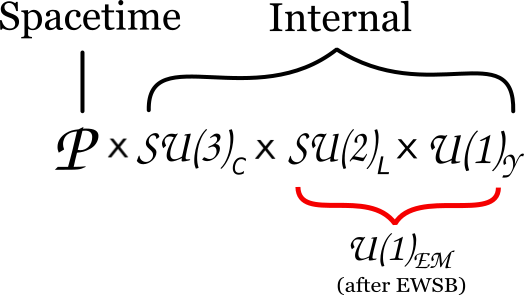
\includegraphics[width=0.5\textwidth]{figures/chapter1/sm_forces}
		\caption{
			The spacetime and internal gauge structure of the SM.
			$\mathcal{P}$ refers to the Poincar{\'e} symmetry group.
			\SUthree$_c$ refers to the \SUthree~symmetry
			of the color sector of QCD and \SUtwo$_{L}\times$\Uone$_{Y}$ refers to the left-handed chiral
			symmetry of the electroweak interaction. After spontaneous symmetry
			breaking due to the Higgs mechanism, the \SUtwo$_L \times$ \Uone$_Y$ symmetry
			reduces to the \Uone$_{EM}$ symmetry of electromagnetism. 
		}
		\label{fig:sm_forces}
	\end{center}
\end{figure}
\FloatBarrier

The SM Lagrangian is shown in Equation \ref{eq:sm_lagrangian} and describes the complete
content of the SM: encompassing all interactions between the known particles and the
symmetries that they obey.

\begin{align}
	\mathcal{L}_{\text{SM}} = -\frac{1}{4} \sum\limits_{\text{gauge}} \mathit{F}_{\mu \nu}^i \mathit{F}^{i\,\mu\nu}
	- \sum\limits_{f} \bar{f}\gamma^{\mu} \mathit{D}_{\mu} f 
	+  (\mathit{D}_{\mu} \phi)^{\dagger} (\mathit{D}^{\mu} \phi) - \mu^2 \phi^{\dagger}\phi - \lambda(\phi^{\dagger}\phi)^2
	\label{eq:sm_lagrangian}
\end{align}
\noindent
The first term of Equation~\ref{eq:sm_lagrangian} is a sum over the three internal gauge groups,  and $\mathit{F}^a_{\mu \nu} = \partial_{\mu} \mathit{A}_{\nu}^a - \partial_{\nu} \mathit{A}_{\mu}^a + g f^{abc} \mathit{A}_{\mu}^{b}\mathit{A}_{\nu}^{c}$, where $\mathit{A}_{\mu}$ is one of the
three gauge fields, $g$ is the associated gauge coupling parameter, and a sum over $i$ is implied. The $f^{abc}$ are the so-called
\textit{structure constants} of the gauge group. For Abelian groups like \Uone, $f^{abc}$ = 0.
For non-Abelian gauge groups like \SUtwo~and \SUthree, $f^{abc} \ne 0$. For example, for
\SUtwo~the structure constants are nothing more than the Levi-Civita totally anti-symmetric tensor, 
$\varepsilon_{ijk}$, giving for the weak gauge force:
\begin{equation}
	\mathbfcal{W}_{\mu \nu} = \partial_{\mu} \mathbfcal{W}_{\nu} - \partial_{\nu} \mathbfcal{W}_{\mu} - g_2 \mathbfcal{W}_{\mu} \times \mathbfcal{W}_{\nu}
\end{equation}
where $\mathbfcal{W}_{\mu}$ is the vector of the three weak gauge fields (\fieldWone, \fieldWtwo, and \fieldWthree) and $g_2$ is their associated gauge coupling. The non-zero $f^{abc}$ of non-Abelian gauge groups means that the gauge bosons of
the weak and strong interactions can interact with themselves due to terms appearing in Equation
\ref{eq:sm_lagrangian} that contain only the gauge bosons. %{\color{red}{add Feynman diagram? -- showing what the squared term of $W_{\mu \nu}$ representing triple and quartic couplings}}

The second term of Equation~\ref{eq:sm_lagrangian} describes the lepton and quark kinetic energies and their interactions with the gauge fields.
The $f$ refer to the fermion fields (quarks and leptons) and the corresponding sum is over all
species of fermion. $\mathit{D}_{\mu}$ is the gauge covariant derivative, and for the SM is
given by:

\begin{equation}
	\mathit{D}_{\mu} = \partial_{\mu} - i g_1 \frac{Y}{2} \mathcal{B}_{\mu} - i g_2 \frac{\tau^i}{2} \mathcal{W}_{\mu}^i - i g_3 \frac{\lambda^a}{2} G_{\mu}^a
	\label{eq:gauge_derivative}
\end{equation}
where $g_1$, $g_2$, and $g_3$ are the gauge coupling constants for \Uone$_{Y}$, \SUtwo$_{L}$, and \SUthree$_{C}$, respectively, that give the overall strength of the associated coupling.
Summation over repeated indices is implied and the $\tau^i$ ($\lambda^a$) are the three (eight)
generators of the \SUtwo~(\SUthree)~gauge group, with $i \in [1,2,3]$ ($a \in [1,..,8]$), and
are typically represented by the Pauli (Gell-Mann) matrices. Note that the form of Equation~\ref{eq:gauge_derivative} is strictly mandated by the requirement that the theory
be \textit{gauge invariant}, i.e. that transformations of the fields under the internal symmetries
of Figure \ref{fig:sm_forces} leave the action of $\mathcal{L}_{\text{SM}}$ unchanged. This is described in detail
in {\color{red}{Appendix XXX}}.

The last three terms in Equation \ref{eq:sm_lagrangian} are all terms including the Higgs field, $\phi$,
and will be discussed in detail in Section~\ref{sec:higgs_description}.

Inspection of Equation~\ref{eq:sm_lagrangian} will reveal two things. The first thing that one
may notice is that it does not appear to describe electromagnetism as it does not have a
term representing the photon, the familiar mediator of the electromagnetic interaction.
The second, and perhaps more immediately obvious, thing is that no mass terms
appear in $\mathcal{L}_{\text{SM}}$: all fields appear to have zero mass! Both of these
facts are counter to our everyday experience: we know electromagnetism is real and that matter,
at the very least, is massive. In the next few sections we will see how these apparent
issues are resolved.


\begin{table}[!htb]
    \caption{
        The particle content of the SM and their transformation
        properties under the SM gauge groups, prior to electroweak symmetry breaking.
        The representations of each of the gauge groups are shown in the three-right
        columns. The \Uone symmetry of weak-hypercharge transformations is one-dimensional
        and the column gives the weak-hypercharge $\mathcal{Y}$ associated with each
        field. For \SUthree and \SUtwo, $\mathbf{1}$ refers to the field belonging to
        the associated singlet representation, $\mathbf{2}$ to the doublet representation,
        $\mathbf{3}$ to the triplet representation, and $\mathbf{8}$ to the octet representation.
    }
    \begin{center}
        \begin{tabularx}{0.96\textwidth}{m{1em} c c c c c c }
        \toprule
        \hline
        & Field Label & Content & Spin & \Uone~($\mathcal{=Y}$) & \SUtwo & \SUthree \\
        \hline
        \rotatebox{90}{\hspace{-0.1cm}\textbf{Quarks} } 
         &   \makecell{\fieldQi \\ \fieldUri \\ \fieldDri} % FIELD
         &   \makecell{ (\fieldUl, \fieldDl), (\fieldCl, \fieldSl), (\fieldTl, \fieldBl) \\ \fieldUr \\ \fieldDr}% CONTENT
         &   \makecell{ $1/2$ \\ $1/2$ \\ $1/2$} % SPIN
         &   \makecell{ $1/6$ \\ $2/3$ \\ $-1/3$}% U(1)
         &   \makecell{ $\mathbf{2}$ \\ $\mathbf{1}$ \\ $\mathbf{1}$}% SU(2)
         &   \makecell{ $\mathbf{3}$ \\ $\mathbf{3}$ \\ $\mathbf{3}$}\\ % SU(3)
        %\cdashline{1-7}
        \rotatebox{90}{\hspace{-0.1cm}\textbf{Leptons} }
         &   \makecell{\fieldLi \\ \fieldEri} % FIELD
         &   \makecell{ (\fieldEl, \fieldNuEl), (\fieldMul, \fieldNuMul), (\fieldTaul, \fieldNuTaul) \\ \fieldEr, \fieldMur, \fieldTaur}% CONTENT
         &   \makecell{ $1/2$ \\ $1/2$ }% SPIN
         &   \makecell{ $1/2$ \\ $-1$ }% U(1)
         &   \makecell{ $\mathbf{2}$ \\ $\mathbf{1}$ }% SU(2)
         &   \makecell{ $\mathbf{1}$ \\ $\mathbf{1}$ } \\ % SU(3)
        \midrule
        \rotatebox{90}{\textbf{\stackanchor{Gauge}{Fields}} }
         &   \makecell{\fieldB \\ \fieldW \\ \fieldG } % FIELD
         &   \makecell{ \fieldB \\ (\fieldWone, \fieldWtwo, \fieldWthree) \\ \fieldG$_a$, $a\in[1,..,8]$ }% CONTENT
         &   \makecell{ $1$ \\ $1$ \\ $1$} % SPIN
         &   \makecell{ $0$ \\ $0$ \\ $0$}% U(1)
         &   \makecell{ $\mathbf{1}$ \\ $\mathbf{3}$ \\ $\mathbf{1}$}% SU(2)
         &   \makecell{ $\mathbf{1}$ \\ $\mathbf{1}$ \\ $\mathbf{8}$}\\ % SU(3)
        \midrule
        \rotatebox{90}{\textbf{\stackanchor{Higgs}{Field}}} 
         &   \makecell{\fieldPhi } % FIELD
         &   \makecell{ (\fieldPhip, \fieldPhizero) }% CONTENT
         &   \makecell{ $0$  } % SPIN
         &   \makecell{ $1/2$  }% U(1)
         &   \makecell{ $\mathbf{2}$ }% SU(2)
         &   \makecell{ $\mathbf{1}$ }\\ % SU(3)
        \hline
        \bottomrule
        \end{tabularx}
    \end{center}
    \label{tab:sm_content}
\end{table}

\FloatBarrier






%\section{Particles and Forces}
%
%Here we introduce the SM particle content and provide a description of the interactions that
%link the particles together.
%
%
\begin{table}[!htb]
    \caption{
        The particle content of the SM and their transformation
        properties under the SM gauge groups, prior to electroweak symmetry breaking.
        The representations of each of the gauge groups are shown in the three-right
        columns. The \Uone symmetry of weak-hypercharge transformations is one-dimensional
        and the column gives the weak-hypercharge $\mathcal{Y}$ associated with each
        field. For \SUthree and \SUtwo, $\mathbf{1}$ refers to the field belonging to
        the associated singlet representation, $\mathbf{2}$ to the doublet representation,
        $\mathbf{3}$ to the triplet representation, and $\mathbf{8}$ to the octet representation.
    }
    \begin{center}
        \begin{tabularx}{0.96\textwidth}{m{1em} c c c c c c }
        \toprule
        \hline
        & Field Label & Content & Spin & \Uone~($\mathcal{=Y}$) & \SUtwo & \SUthree \\
        \hline
        \rotatebox{90}{\hspace{-0.1cm}\textbf{Quarks} } 
         &   \makecell{\fieldQi \\ \fieldUri \\ \fieldDri} % FIELD
         &   \makecell{ (\fieldUl, \fieldDl), (\fieldCl, \fieldSl), (\fieldTl, \fieldBl) \\ \fieldUr \\ \fieldDr}% CONTENT
         &   \makecell{ $1/2$ \\ $1/2$ \\ $1/2$} % SPIN
         &   \makecell{ $1/6$ \\ $2/3$ \\ $-1/3$}% U(1)
         &   \makecell{ $\mathbf{2}$ \\ $\mathbf{1}$ \\ $\mathbf{1}$}% SU(2)
         &   \makecell{ $\mathbf{3}$ \\ $\mathbf{3}$ \\ $\mathbf{3}$}\\ % SU(3)
        %\cdashline{1-7}
        \rotatebox{90}{\hspace{-0.1cm}\textbf{Leptons} }
         &   \makecell{\fieldLi \\ \fieldEri} % FIELD
         &   \makecell{ (\fieldEl, \fieldNuEl), (\fieldMul, \fieldNuMul), (\fieldTaul, \fieldNuTaul) \\ \fieldEr, \fieldMur, \fieldTaur}% CONTENT
         &   \makecell{ $1/2$ \\ $1/2$ }% SPIN
         &   \makecell{ $1/2$ \\ $-1$ }% U(1)
         &   \makecell{ $\mathbf{2}$ \\ $\mathbf{1}$ }% SU(2)
         &   \makecell{ $\mathbf{1}$ \\ $\mathbf{1}$ } \\ % SU(3)
        \midrule
        \rotatebox{90}{\textbf{\stackanchor{Gauge}{Fields}} }
         &   \makecell{\fieldB \\ \fieldW \\ \fieldG } % FIELD
         &   \makecell{ \fieldB \\ (\fieldWone, \fieldWtwo, \fieldWthree) \\ \fieldG$_a$, $a\in[1,..,8]$ }% CONTENT
         &   \makecell{ $1$ \\ $1$ \\ $1$} % SPIN
         &   \makecell{ $0$ \\ $0$ \\ $0$}% U(1)
         &   \makecell{ $\mathbf{1}$ \\ $\mathbf{3}$ \\ $\mathbf{1}$}% SU(2)
         &   \makecell{ $\mathbf{1}$ \\ $\mathbf{1}$ \\ $\mathbf{8}$}\\ % SU(3)
        \midrule
        \rotatebox{90}{\textbf{\stackanchor{Higgs}{Field}}} 
         &   \makecell{\fieldPhi } % FIELD
         &   \makecell{ (\fieldPhip, \fieldPhizero) }% CONTENT
         &   \makecell{ $0$  } % SPIN
         &   \makecell{ $1/2$  }% U(1)
         &   \makecell{ $\mathbf{2}$ }% SU(2)
         &   \makecell{ $\mathbf{1}$ }\\ % SU(3)
        \hline
        \bottomrule
        \end{tabularx}
    \end{center}
    \label{tab:sm_content}
\end{table}

%
\begin{table}[!htb]
    \caption{
        The particle content of the SM after the process of
        electroweak symmetry breaking.
    }
    \begin{center}
        \begin{tabularx}{1\textwidth}{m{1em} c c c c }
        \toprule
        \hline
        & Physical Field & Q & Coupling & Mass [GeV] \\
        \hline
        \rotatebox{90}{\hspace{-0.1cm}\textbf{Quarks} } 
            & \makecell{ \quarkU, \quarkC, \quarkT \\ \quarkD, \quarkS, \quarkB} % FIELD
            & \makecell{ $2/3$ \\ $-1/3$ }% Q
            %& \makecell{ $\mathbf{3}$ \\ $\mathbf{3}$ } % SU(3)
            & \makecell{ ($y_i=$) $1\times10^{-5}$, $7\times10^{-3}$, $1$ \\ ($y_i=$) $3\times10^{-5}$, $5\times10^{-4}$, $0.02$ } % Coupling
            & \makecell{ $2\times10^{-3}$, $1.27$, $173$ \\ $4\times10^{-4}$, $0.10$, $4.18$ }\\% Mass
        \rotatebox{90}{\hspace{-0.1cm}\textbf{Leptons} } 
            & \makecell{ \leptonE, \leptonMu, \leptonTau \\ \neutrinoE, \neutrinoMu, \neutrinoTau } % FIELD
            & \makecell{ $-1$ \\ $0$ }% Q
            %& \makecell{ $\mathbf{1}$ \\ $\mathbf{1}$ } % SU(3)
            & \makecell{ ($y_i=$) $3\times10^{-7}$, $6\times10^{-4}$, $0.01$ \\ -- } % Coupling
            & \makecell{ $5\times10^{-4}$, $0.106$, $1.777$ \\ --}\\% Mass
        \midrule
        \rotatebox{90}{\textbf{Bosons} } 
            & \makecell{ \fieldPhoton \\ \fieldZ \\ (\fieldWp, \fieldWm) \\ \fieldG } % FIELD
            & \makecell{ $0$ \\ $0$ \\ $(+1,-1)$ \\ $0$ }% Q
            %& \makecell{ $\mathbf{1}$ \\ $\mathbf{1}$ \\ $\mathbf{1}$ \\ $\mathbf{8}$ } % SU(3)
            & \makecell{ $\alpha_{\text{EM}} \simeq 1/137$ \\ $\sin \theta_{W} \simeq 0.5$ \\ -- \\ $\alpha_s \simeq 0.1$ } % Coupling
            & \makecell{ $0$ \\ $91.2$ \\ $80.4$ \\  $0$}\\% Mass
        \midrule
        \rotatebox{90}{\textbf{Higgs} } 
            & \makecell{ \fieldH } % FIELD
            & \makecell{ $0$ }% Q
            %& \makecell{ $\mathbf{1}$ } % SU(3)
            & \makecell{ $\lambda$, $\mu$ } % Coupling
            & \makecell{ $125.09$ }\\% Mass

         %&   \makecell{ (\quarkUl, \quarkDl), (\quarkCl, \quarkSl), (\quarkTl, \quarkBl) \\ \quarkUr \\ \quarkDr}% CONTENT
         %&   \makecell{ $1/2$ \\ $1/2$ \\ $1/2$} % SPIN
         %&   \makecell{ $\mathbf{2}$ \\ $\mathbf{1}$ \\ $\mathbf{1}$}% SU(2)
         %&   \makecell{ $\mathbf{3}$ \\ $\mathbf{3}$ \\ $\mathbf{3}$}\\ % SU(3)
        %%\cdashline{1-7}
        %rotatebox{90}{\hspace{-0.1cm}\textbf{Leptons} }
         %&   \makecell{\quarkLi \\ \quarkEri} % FIELD
         %&   \makecell{ (\quarkEl, \quarkNuEl), (\quarkMul, \quarkNuMul), (\quarkTaul, \quarkNuTaul) \\ \quarkEr, \quarkMur, \quarkTaur}% CONTENT
         %&   \makecell{ $1/2$ \\ $1/2$ }% SPIN
         %&   \makecell{ $\mathbf{2}$ \\ $\mathbf{1}$ }% SU(2)
         %&   \makecell{ $\mathbf{1}$ \\ $\mathbf{1}$ } \\ % SU(3)
        %midrule
        %rotatebox{90}{\textbf{\stackanchor{Gauge}{Fields}} }
         %&   \makecell{\quarkB \\ \quarkW \\ \quarkG } % FIELD
         %&   \makecell{ \quarkB \\ (\quarkWone, \quarkWtwo, \quarkWthree) \\ \quarkG }% CONTENT
         %&   \makecell{ $1$ \\ $1$ \\ $1$} % SPIN
         %&   \makecell{ $\mathbf{1}$ \\ $\mathbf{3}$ \\ $\mathbf{1}$}% SU(2)
         %&   \makecell{ $\mathbf{1}$ \\ $\mathbf{1}$ \\ $\mathbf{8}$}\\ % SU(3)
        %midrule
        %rotatebox{90}{\textbf{\stackanchor{Higgs}{Field}}} 
         %&   \makecell{\quarkPhi } % FIELD
         %&   \makecell{ (\quarkPhip, \quarkPhizero) }% CONTENT
         %&   \makecell{ $0$  } % SPIN
         %&   \makecell{ $\mathbf{2}$ }% SU(2)
         %&   \makecell{ $\mathbf{1}$ }\\ % SU(3)
        \hline
        \bottomrule
        \end{tabularx}
    \end{center}
    \label{tab:sm_content}
\end{table}



%\subsection{Gauge Theories}

%\subsubsection{The Electroweak Theory}


